\subsubsection{Công nghệ Front-end}

\subsubsubsection{ReactJS}
    \begin{enumerate}[(a)]
        \item \textit{Giới thiệu}
        
            ReactJS là một thư viện JavaScript mã nguồn mở, được phát triển bởi Facebook, nhằm hỗ trợ xây dựng giao diện người dùng (UI) cho các ứng dụng web. Ra mắt vào năm 2013, ReactJS nhanh chóng trở thành một trong những công cụ phổ biến nhất cho việc phát triển UI tương tác và hiệu quả.
            
            % Các đặc điểm nổi bật của ReactJS:
    
            % \begin{itemize}
            %     \item \textbf{Kiến trúc dựa trên thành phần (Component-Based Architecture)}: React cho phép chia UI thành các thành phần nhỏ, độc lập và có thể tái sử dụng. Mỗi thành phần quản lý trạng thái và logic riêng, giúp việc phát triển và bảo trì ứng dụng trở nên dễ dàng hơn.
            %     \item \textbf{Virtual DOM}: React sử dụng một bản sao ảo của DOM thật, gọi là Virtual DOM. Khi có sự thay đổi trong trạng thái hoặc dữ liệu, React cập nhật Virtual DOM trước, sau đó so sánh với DOM thật và chỉ thực hiện những thay đổi cần thiết. Điều này cải thiện hiệu suất và tăng tốc độ render của ứng dụng.
            %     \item \textbf{JSX (JavaScript XML)}: React sử dụng JSX, một cú pháp mở rộng cho phép viết mã HTML trong JavaScript. Điều này giúp code trở nên dễ đọc và dễ hiểu hơn, đồng thời tối ưu hóa quá trình phát triển UI.
            %     \item \textbf{One-way Data Binding}: React áp dụng cơ chế liên kết dữ liệu một chiều, giúp luồng dữ liệu trở nên rõ ràng và dễ kiểm soát. Dữ liệu được truyền từ component cha đến component con thông qua props, giúp việc quản lý và debug ứng dụng trở nên hiệu quả hơn. 
            % \end{itemize}

        
        \item \textit{Ưu điểm} \cite{React}.

        \begin{itemize}
            \item  \textbf{Khai báo giao diện (Declarative)}: React giúp tạo ra các giao diện người dùng tương tác một cách dễ dàng. Bằng cách thiết kế các khung nhìn cho từng trạng thái trong ứng dụng, React sẽ tự động cập nhật và render các thành phần phù hợp khi dữ liệu thay đổi. Việc khai báo giao diện một cách tường minh giúp mã nguồn dễ hiểu và dễ dàng gỡ lỗi hơn.
            \item \textbf{Component-Based}: React cho phép xây dựng các thành phần độc lập và quản lý trạng thái riêng biệt của chúng. Những thành phần này có thể được kết hợp để tạo ra các giao diện phức tạp. Việc viết logic của thành phần bằng JavaScript thay vì template giúp dễ dàng truyền dữ liệu và tránh thao tác trực tiếp với DOM.
            \item \textbf{Học một lần, viết ở mọi nơi (Learn Once, Write Anywhere)}: React không phụ thuộc vào kỹ năng công nghệ cụ thể, cho phép phát triển các tính năng mới mà không cần viết lại mã hiện có. React có thể render trên máy chủ bằng Node.js và xây dựng ứng dụng di động thông qua React Native 
        \end{itemize}

        \item \textit{So sánh React và các công nghệ khác} 
        
            Khi so sánh giữa các công nghệ phổ biến hiện nay như ReactJS, Angular, Vue.js và Svelte, chúng ta có thể thấy những đặc điểm riêng biệt của từng công nghệ, giúp lựa chọn được công nghệ phù hợp với nhu cầu và yêu cầu của dự án. Dựa theo tài liệu \cite{FrontCompare1} và \cite{FrontCompare2}, dưới đây là bảng so sánh chi tiết giữa ReactJS và các công nghệ khác:

            % \begin{longtable}{|p{3.5cm}|p{5.5cm}|p{5.5cm}|}
            % \hline
            % \textbf{Tiêu Chí} & \textbf{ReactJS} & \textbf{Angular} \\ 
            % \hline
            % \endfirsthead
            % \hline
            % \textbf{Tiêu Chí} & \textbf{ReactJS} & \textbf{Angular} \\ 
            % \endhead
            % \hline
            % % \multicolumn{3}{|r|}{\small\slshape Còn tiếp} \\ \hline
            % \endfoot
            % \hline
            % \endlastfoot
            % Ngôn ngữ & JavaScript (hỗ trợ TypeScript)     & TypeScript (bắt buộc)\\ 
            % \hline
            % Định nghĩa & Thư viện JavaScript để xây dựng giao diện người dùng & Framework toàn diện để phát triển ứng dụng web\\ 
            % \hline
            % Kiến trúc & Dựa trên thành phần, Virtual DOM, luồng dữ liệu một chiều & Dựa trên thành phần, MVC/MVVM, cơ chế phát hiện thay đổi\\ 
            % \hline
            % Thời gian phát triển & Nhanh cho dự án nhỏ, chậm hơn nếu cần tích hợp nhiều thư viện & Chậm hơn do cấu hình ban đầu phức tạp, nhanh cho dự án lớn nhờ tích hợp sẵn\\ 
            % \hline
            % Độ phức tạp & Trung bình, phụ thuộc vào cách quản lý trạng thái & Cao, nhiều khái niệm (Dependency Injection, RxJS, Modules)\\ 
            % \hline
            % Tính linh hoạt & Cao, tự do chọn thư viện và công cụ & Thấp hơn, bị ràng buộc bởi cấu trúc framework\\ 
            % \hline
            % Bảo trì & Dễ bảo trì với các thành phần nhỏ & Dễ bảo trì cho dự án lớn, khó hơn với dự án nhỏ do cấu trúc phức tạp\\ 
            % \hline
            % Dễ sử dụng/Dễ học & Dễ học với người biết JavaScript & Khó học, cần hiểu TypeScript và các khái niệm framework\\ 
            % \hline
            % Hỗ trợ cộng đồng & Rất lớn, nhiều tài liệu, thư viện và diễn đàn & Lớn, hỗ trợ chính thức từ Google, tài liệu chi tiết\\ 
            % \hline
            % Kiểm thử & Jest, React Testing Library, dễ thiết lập & Jasmine, Karma, tích hợp sẵn nhưng phức tạp hơn\\ 
            % \hline
            % \caption{Bảng so sánh ReactJS và Angular}\\
            % \end{longtable}

            % \begin{longtable}{|p{3.5cm}|p{5.5cm}|p{5.5cm}|}
            % \hline
            % \textbf{Tiêu Chí} & \textbf{Svelt} & \textbf{Vue.js} \\ 
            % \hline
            % \endfirsthead
            % \hline
            % \textbf{Tiêu Chí} & \textbf{Svelt} & \textbf{Vue.js} \\ 
            % \endhead
            % \hline
            % % \multicolumn{3}{|r|}{\small\slshape Còn tiếp} \\ \hline
            % \endfoot
            % \hline
            % \endlastfoot
            % Ngôn ngữ & JavaScript (hỗ trợ TypeScript)     & JavaScript (hỗ trợ TypeScript)\\ 
            % \hline
            % Định nghĩa & Framework biên dịch, chuyển mã thành Vanilla JS & Framework tiến bộ để xây dựng giao diện người dùng\\ 
            % \hline
            % Kiến trúc & Dựa trên thành phần, hệ thống phản ứng tích hợp sẵn, không dùng Virtual DOM & Dựa trên thành phần, hệ thống phản ứng, Virtual DOM\\ 
            % \hline
            % Thời gian phát triển & Nhanh, nhờ cú pháp đơn giản và không cần runtime & Nhanh, nhờ cú pháp dễ hiểu và tích hợp tốt với các công cụ\\ 
            % \hline
            % Độ phức tạp & Thấp, ít khái niệm phức tạp & Trung bình, phức tạp hơn khi dùng Vuex hoặc các tính năng nâng cao\\ 
            % \hline
            % Tính linh hoạt & Trung bình, ít tùy chỉnh hơn do biên dịch & Cao, dễ tích hợp với nhiều thư viện và công cụ\\ 
            % \hline
            % Bảo trì & Dễ bảo trì nhờ mã biên dịch sạch, ít lỗi runtime & Dễ bảo trì với dự án nhỏ, phức tạp hơn với dự án lớn nếu không tổ chức tốt\\ 
            % \hline
            % Dễ sử dụng/Dễ học & Rất dễ học, gần với HTML, CSS, JS truyền thống & Dễ học, cú pháp trực quan, phù hợp với cả người mới và chuyên gia\\ 
            % \hline
            % Hỗ trợ cộng đồng & Nhỏ hơn, đang phát triển, ít tài liệu hơn & Lớn, năng động, nhiều tài liệu và tài nguyên\\ 
            % \hline
            % Kiểm thử & Vitest, Playwright, đơn giản nhưng ít tài liệu & Jest, Vue Test Utils, dễ thiết lập và có cộng đồng hỗ trợ\\ 
            % \hline
            % \caption{Bảng so sánh Svelt và Vue.js}\\
            % \end{longtable}

            \newpage

\begin{landscape}  % Bắt đầu phần landscape
\begin{longtable}{|p{3.5cm}|p{5cm}|p{5cm}|p{5cm}|p{5cm}|}
\hline
\textbf{Tiêu Chí} & \textbf{ReactJS} & \textbf{Angular} & \textbf{Svelt} & \textbf{Vue.js} \\
\hline
\endfirsthead
\hline
\textbf{Tiêu Chí} & \textbf{ReactJS} & \textbf{Angular} & \textbf{Svelt} & \textbf{Vue.js} \\
\hline
\endhead
\hline
Ngôn ngữ & JavaScript (hỗ trợ TypeScript) & TypeScript (bắt buộc) & JavaScript (hỗ trợ TypeScript) & JavaScript (hỗ trợ TypeScript) \\
\hline
Định nghĩa & Thư viện JavaScript để xây dựng giao diện người dùng & Framework toàn diện để phát triển ứng dụng web & Framework biên dịch, chuyển mã thành Vanilla JS & Framework tiến bộ để xây dựng giao diện người dùng \\
\hline
Kiến trúc & Dựa trên thành phần, Virtual DOM, luồng dữ liệu một chiều & Dựa trên thành phần, MVC/MVVM, cơ chế phát hiện thay đổi & Dựa trên thành phần, hệ thống phản ứng tích hợp sẵn, không dùng Virtual DOM & Dựa trên thành phần, hệ thống phản ứng, Virtual DOM \\
\hline
Thời gian phát triển & Nhanh cho dự án nhỏ, chậm hơn nếu cần tích hợp nhiều thư viện & Chậm hơn do cấu hình ban đầu phức tạp, nhanh cho dự án lớn nhờ tích hợp sẵn & Nhanh, nhờ cú pháp đơn giản và không cần runtime & Nhanh, nhờ cú pháp dễ hiểu và tích hợp tốt với các công cụ \\
\hline
Độ phức tạp & Trung bình, phụ thuộc vào cách quản lý trạng thái & Cao, nhiều khái niệm (Dependency Injection, RxJS, Modules) & Thấp, ít khái niệm phức tạp & Trung bình, phức tạp hơn khi dùng Vuex hoặc các tính năng nâng cao \\
\hline
Tính linh hoạt & Cao, tự do chọn thư viện và công cụ & Thấp hơn, bị ràng buộc bởi cấu trúc framework & Trung bình, ít tùy chỉnh hơn do biên dịch & Cao, dễ tích hợp với nhiều thư viện và công cụ \\
\hline
Bảo trì & Dễ bảo trì với các thành phần nhỏ & Dễ bảo trì cho dự án lớn, khó hơn với dự án nhỏ do cấu trúc phức tạp & Dễ bảo trì nhờ mã biên dịch sạch, ít lỗi runtime & Dễ bảo trì với dự án nhỏ, phức tạp hơn với dự án lớn nếu không tổ chức tốt \\
\hline
Dễ sử dụng/Dễ học & Dễ học với người biết JavaScript & Khó học, cần hiểu TypeScript và các khái niệm framework & Rất dễ học, gần với HTML, CSS, JS truyền thống & Dễ học, cú pháp trực quan, phù hợp với cả người mới và chuyên gia \\
\hline
Kiểm thử & Jest, React Testing Library, dễ thiết lập & Jasmine, Karma, tích hợp sẵn nhưng phức tạp hơn & Vitest, Playwright, đơn giản nhưng ít tài liệu & Jest, Vue Test Utils, dễ thiết lập và có cộng đồng hỗ trợ \\
\hline
\caption{Bảng so sánh các công nghệ Front-end phổ biến}
\end{longtable}
\end{landscape}
            
            Ngoài ra, theo các dữ liệu về xu hướng công nghệ từ Stack Overflow \cite{FrontendFrameworks}, với việc theo dõi mức độ sử dụng tag từ năm 2008 - khi nền tảng này được ra mắt - ReactJS vẫn luôn duy trì vị trí hàng đầu cho đến nay.

            \begin{figure}[H]
                \centering
                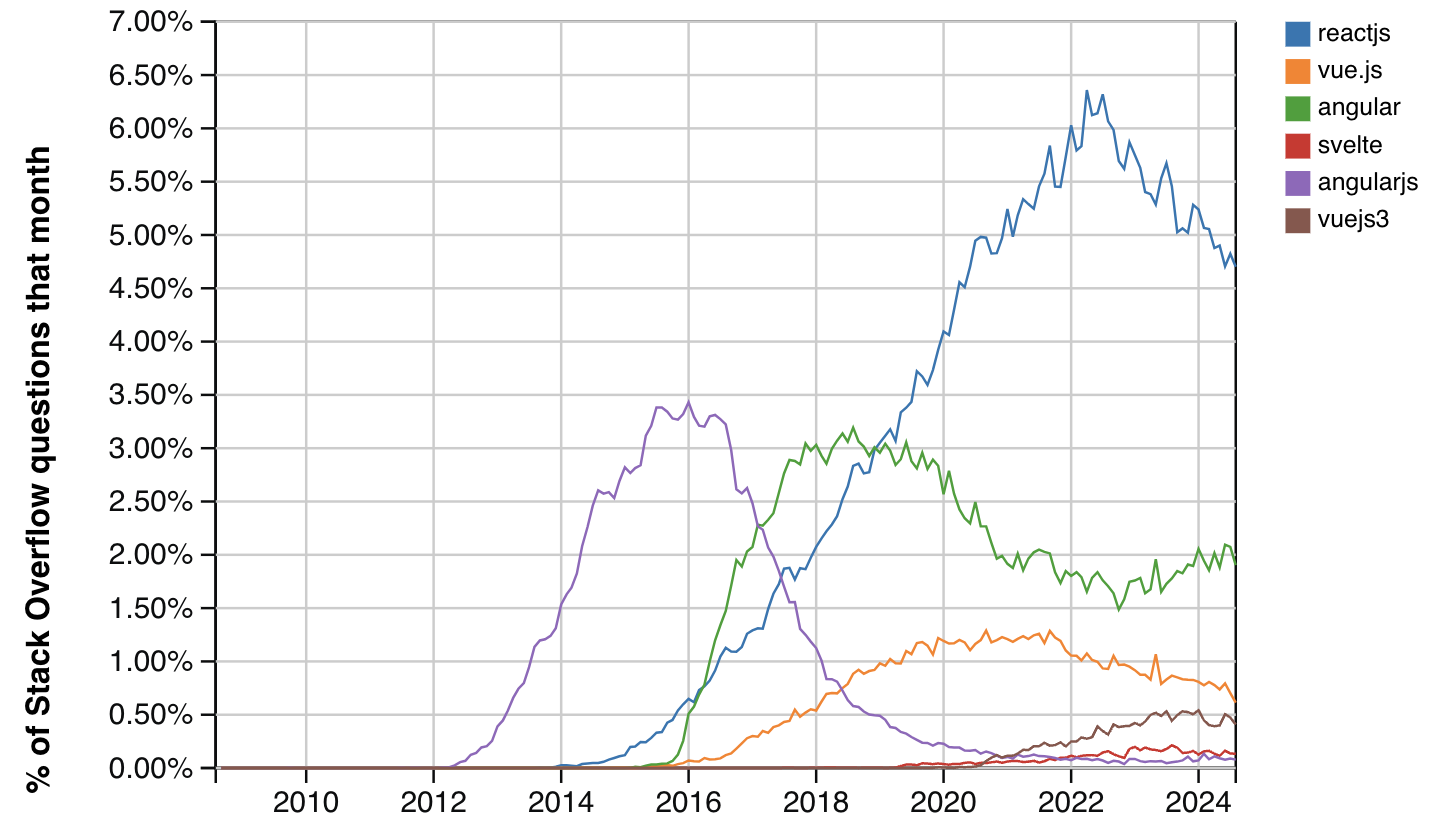
\includegraphics[width=10cm]{Images/react-stack-overflow.png}
                \vspace{0.5cm}
                \caption{Đồ thị phần trăm việc sử dụng tag tên trên Stackoverflow. Truy cập ngày: 13/02/2025}
                \label{fig:my_label}
            \end{figure}

            \textbf{Kết luận: } Dựa trên các bảng so sánh, nhóm quyết định chọn ReactJS là công nghệ chính để phát triển giao diện người dùng vì các lý do sau:

            \begin{itemize}
                \item Phù hợp với quy mô dự án: ReactJS không yêu cầu cấu trúc quá phức tạp như Angular, rất phù hợp với các dự án vừa và nhỏ. Điều này cho phép nhóm tập trung vào tính năng chính, như giao diện đặt món, mà không bị phân tâm vào các chi tiết kỹ thuật phức tạp.
                \item Sự quen thuộc: Việc đã có kinh nghiệm với ReactJS giúp nhóm phát triển hệ thống nhanh chóng hơn, đồng thời có thể tận dụng cộng đồng hỗ trợ lớn từ ReactJS.
            \end{itemize}
            % Dựa trên số liệu từ tháng 1 năm 2020 đến tháng 7 năm 2022, React đã thể hiện sự thống trị vượt trội trong cộng đồng phát triển frontend. Sự phổ biến của React được thể hiện qua số lượng repository phụ thuộc vào nó trên GitHub, vượt xa so với các framework khác như Vue và Angular 2+. Cụ thể, React đã đạt hơn 200.000 lượt sao trên GitHub, trong khi Vue và Angular còn chưa tới 100.000 lượt sao trên GitHub.

            % \begin{figure}[H]
            %     \centering
            %     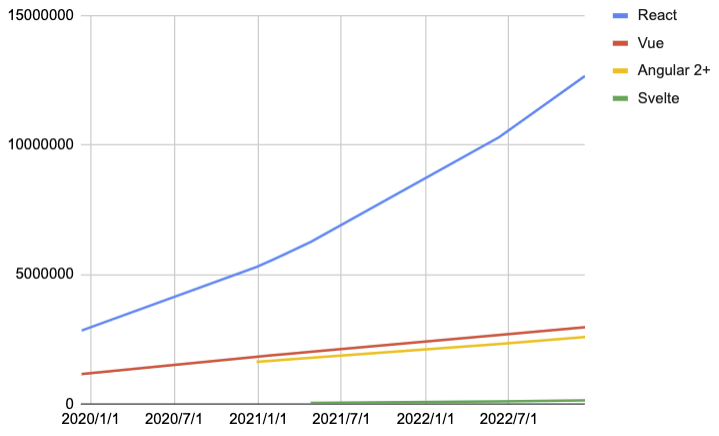
\includegraphics[width=10cm]{Images/react-repository.png}
            %     \vspace{0.5cm}
            %     \caption{Biểu đồ đường số lượng repository sử dụng framework}
            %     \label{fig:my_label}
            % \end{figure}

            % \begin{figure}[H]
            %     \centering
            %     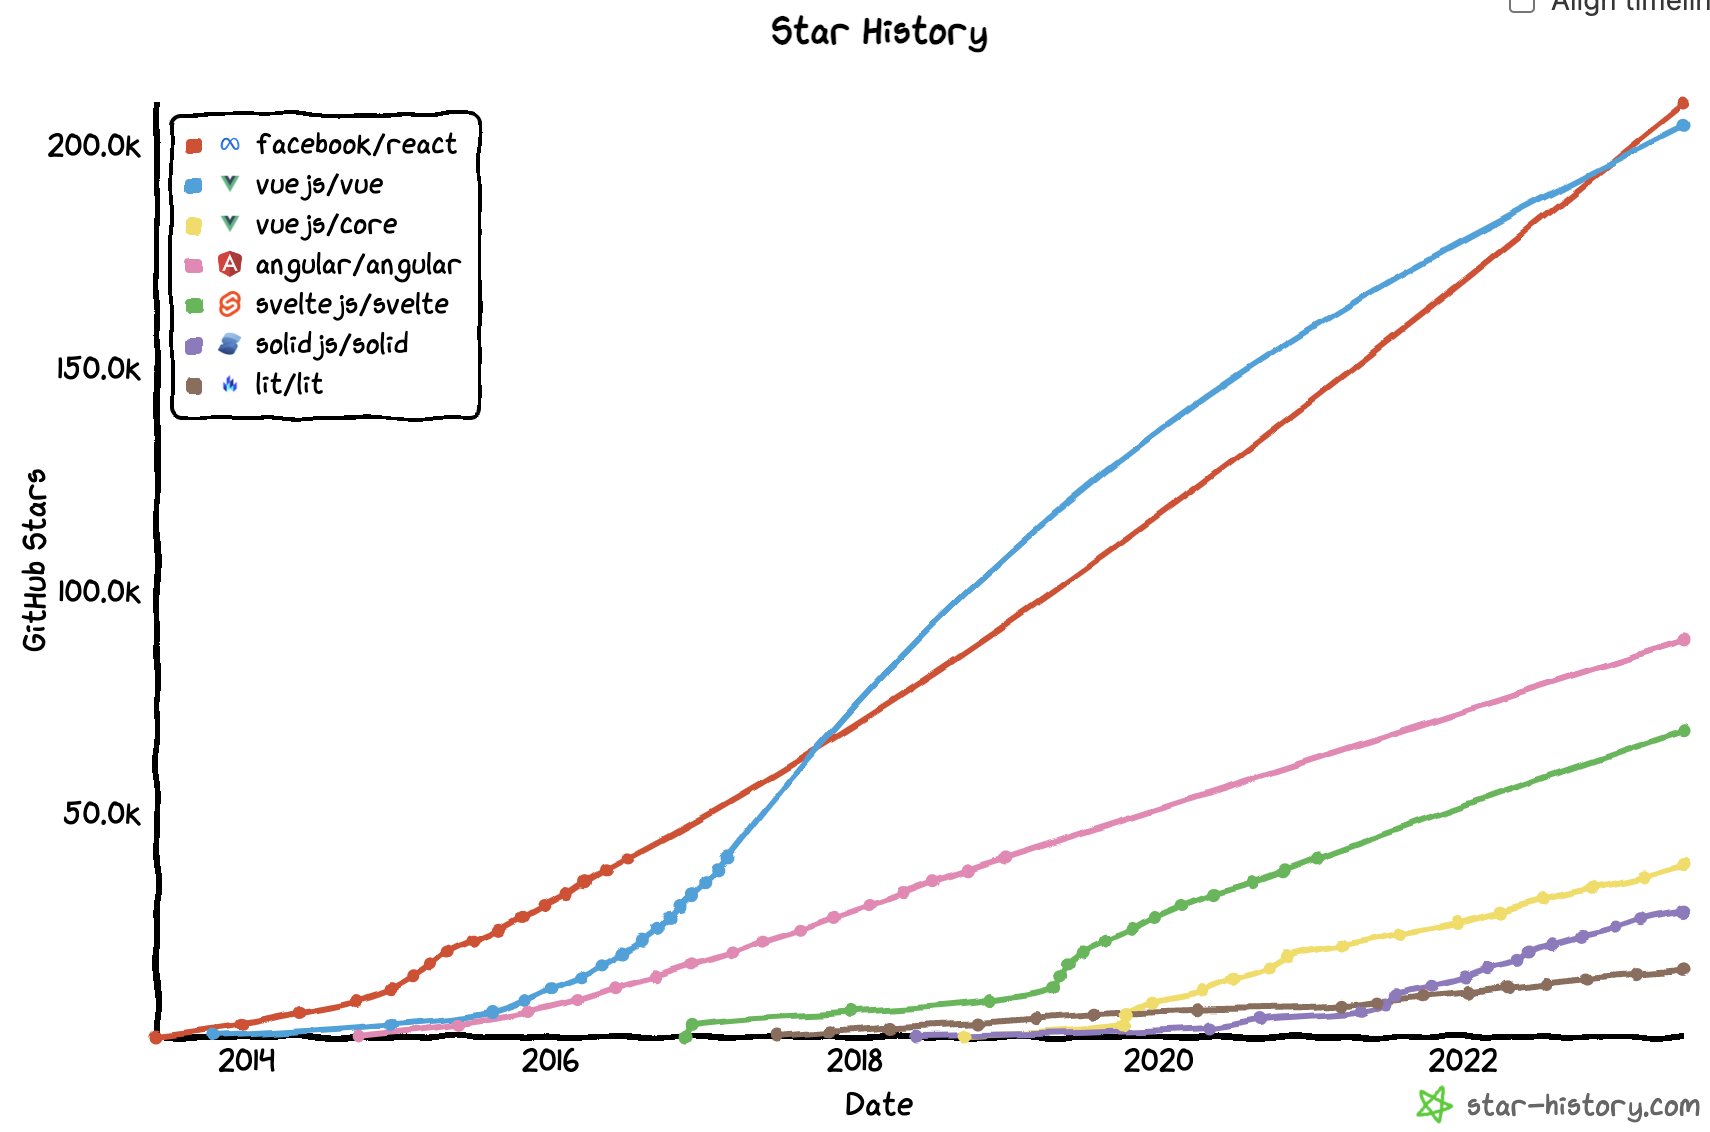
\includegraphics[width=10cm]{Images/react-star-history.png}
            %     \vspace{0.5cm}
            %     \caption{Biểu đồ thống kê GitHub Stars các framework phổ biến}
            %     \label{fig:my_label}
            % \end{figure}
            
            % Và còn nhiều kết quả thống kê khác đều chứng minh React luôn đi đầu trong số các Frontend framework khác như Vue, Angular hay Svelte \cite{FrontendFrameworks}. 
        
        % \item \textit{Nhược điểm}
        % \begin{itemize}
        %     \item \textbf{Vấn đề hiệu suất trên thiết bị cũ}: Ứng dụng React có thể gặp khó khăn trong việc duy trì hiệu suất trên các thiết bị cũ hoặc cấu hình thấp, do việc sử dụng Virtual DOM và các tính năng phức tạp có thể tiêu tốn tài nguyên hệ thống. 
        %     \item \textbf{Cập nhật thường xuyên}: React phát triển nhanh chóng, với các bản cập nhật và tính năng mới liên tục. Điều này có thể tạo ra gánh nặng cho các nhà phát triển trong việc duy trì và cập nhật mã nguồn để tương thích với các phiên bản mới.
        %     \item \textbf{JSX Learning Curve}: JSX, cú pháp kết hợp giữa JavaScript và HTML, có thể gây khó khăn cho những người mới bắt đầu, đặc biệt là khi làm quen với các khái niệm như state, props và lifecycle methods.
        % \end{itemize}
    \end{enumerate}

\subsubsubsection{ShadCN}
    \begin{enumerate}[(a)]
        \item \textit{Giới thiệu}

            ShadCN là một bộ sưu tập các thành phần giao diện người dùng (UI components) có thể tái sử dụng, được thiết kế đẹp mắt và dễ dàng tích hợp vào ứng dụng.

            Được xây dựng dựa trên thư viện Radix và framework Tailwind CSS, ShadCN cung cấp các thành phần như Button, Modal, Dropdown và nhiều hơn nữa, với khả năng tùy chỉnh linh hoạt để phù hợp với nhu cầu của từng dự án.

        \item \textit{Ưu điểm}

        \begin{itemize}
            \item \textbf{Thiết kế hướng đến doanh nghiệp}: ShadCN tập trung vào giao diện người dùng sạch sẽ và chuyên nghiệp, phù hợp cho các công cụ nội bộ và các ứng dụng nghiêm túc.
            \item \textbf{Tích hợp dễ dàng với React}: ShadCN UI được xây dựng đặc biệt cho React, giúp việc tích hợp và sử dụng trong các dự án React trở nên đơn giản và trực quan hơn. Điều này giúp giảm thiểu thời gian học tập và triển khai cho các nhà phát triển React.
            \item \textbf{Hiệu suất tối ưu}: Thư viện được thiết kế để tối ưu hóa hiệu suất, giúp giảm thiểu kích thước gói và tăng tốc độ tải trang. Điều này đặc biệt quan trọng trong các ứng dụng web hiện đại, nơi hiệu suất là yếu tố quan trọng.
        \end{itemize}

        \item \textit{Vì sao chọn ShadCN} 

            Nhóm quyết định chọn ShadCN để phát triển hệ thống Menu+ vì những lý do chính sau:

            \begin{itemize}
                \item Giao diện đồng nhất: ShadCN giúp hệ thống có giao diện đẹp, chuyên nghiệp và nhất quán, mang lại trải nghiệm mượt mà cho người dùng.
                \item Tăng tốc phát triển front-end: Với các thành phần UI đã được thiết kế sẵn, ShadCN giúp giảm thời gian phát triển, cho phép tập trung vào chức năng chính của hệ thống. Bên cạnh đó, nó còn hỗ trợ tính năng responsive, đảm bảo trải nghiệm người dùng trên mọi nền tảng.
                \item Tùy chỉnh dễ dàng: ShadCN cho phép tùy biến giao diện linh hoạt, giúp hệ thống có thể thay đổi theo nhu cầu và yêu cầu cụ thể.
            \end{itemize}

            Về mặt sử dụng, ShadCN hiện đang được sử dụng bởi khoảng 11.395 trang web, trong đó có 14 trang web nằm trong top 10 nghìn.

            \begin{figure}[H]
                \centering
                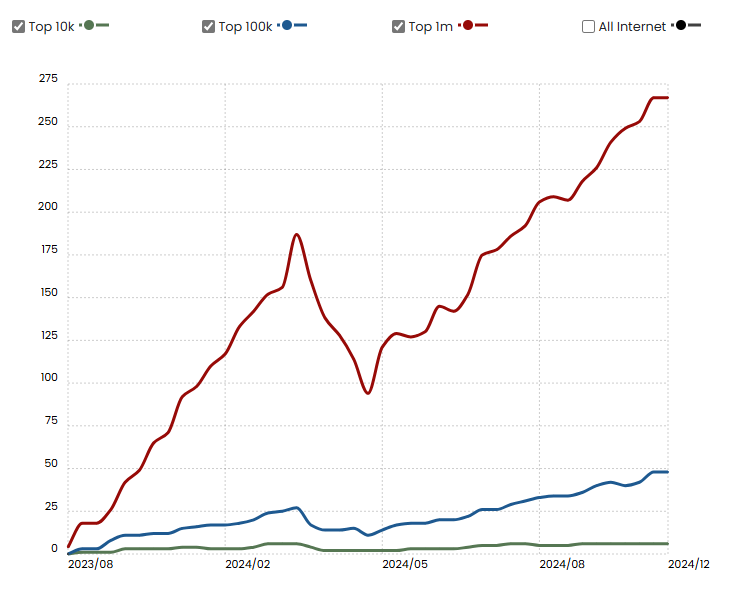
\includegraphics[width=10cm]{Images/shadcn-stats.png}
                \vspace{0.5cm}
                \caption{Thống kê sử dụng shadcn ui \cite{ShadcnUI}}
                \label{fig:my_label}
            \end{figure}
            
        % \item \textit{Nhược điểm}

        % \begin{itemize}
        %     \item \textbf{Thiếu cộng đồng lớn}: So với các thư viện UI phổ biến như MUI, ShadCN UI có cộng đồng người dùng và nhà phát triển nhỏ hơn. Điều này có thể dẫn đến việc thiếu tài liệu hỗ trợ và ít giải pháp cho các vấn đề thường gặp.
        %     \item \textbf{Hạn chế về thành phần giao diện}: Mặc dù ShadCN UI cung cấp nhiều thành phần cơ bản, nhưng so với MUI, thư viện này có thể thiếu một số thành phần phức tạp hoặc đặc biệt, điều này có thể yêu cầu bạn tự phát triển hoặc tích hợp thêm các thư viện khác.
        % \end{itemize}
    \end{enumerate}

\subsubsubsection{TanStack}
    \begin{enumerate}[(a)]
        \item \textit{Giới thiệu}

            TanStack là một tập hợp các thư viện mã nguồn mở chất lượng cao, được thiết kế để hỗ trợ các nhà phát triển web trong việc xây dựng ứng dụng hiệu quả và mạnh mẽ. Các thư viện của TanStack tập trung vào việc cung cấp các tiện ích "headless" (không có giao diện mặc định), an toàn về kiểu dữ liệu và mạnh mẽ cho các tác vụ như quản lý trạng thái, định tuyến, hiển thị dữ liệu và hơn thế nữa.

            TanStack cam kết cung cấp các công cụ mạnh mẽ và linh hoạt, giúp các nhà phát triển tạo ra các ứng dụng web hiệu quả và dễ bảo trì. Với triết lý "headless", các thư viện của TanStack cho phép tùy chỉnh giao diện hoàn toàn, dễ dàng tích hợp vào bất kỳ dự án nào mà không bị ràng buộc bởi các thiết kế mặc định \cite{TanStack}.
        
        \item \textit{Ưu điểm}

        \begin{itemize}
            \item \textbf{Quản lý trạng thái máy chủ hiệu quả}: TanStack Query (trước đây là React Query) giúp quản lý trạng thái bất đồng bộ trong React, đặc biệt trong việc fetching, caching và đồng bộ hóa dữ liệu từ server. Điều này giúp cải thiện hiệu suất và trải nghiệm người dùng.
            \item \textbf{Tối ưu hóa hiệu suất}: Với cơ chế caching tự động, TanStack giảm tải cho server và tăng tốc độ phản hồi của ứng dụng. Dữ liệu được lưu trữ trong bộ nhớ đệm và cập nhật nền, đảm bảo người dùng luôn có thông tin mới nhất mà không cần thực hiện các yêu cầu API không cần thiết. 
            \item \textbf{Xử lý lỗi và quản lý truy vấn dễ dàng}: TanStack cung cấp cách tiếp cận rõ ràng và nhất quán để xử lý lỗi, bao gồm khả năng tự động thử lại các truy vấn HTTP thất bại. Ngoài ra, việc quản lý truy vấn trở nên dễ dàng hơn với các tính năng như nhóm truy vấn, vô hiệu hóa và tìm nạp lại khi cần thiết.
        \end{itemize}

        \item \textit{Vì sao chọn TanStack} 

            TanStack được chọn để phát triển hệ thống Menu+ bởi các lí do chính sau:
            \begin{itemize}
                \item Quản lý trạng thái hiệu quả: TanStack giúp đồng bộ dữ liệu giữa các trang như thực đơn, đơn hàng, và thông tin khách hàng, đảm bảo trải nghiệm người dùng mượt mà. 
                \item Tối ưu hiệu suất: Tính năng caching và prefetching giúp giảm số lần gọi API, tăng tốc độ xử lý dữ liệu như thông tin món ăn, đơn hàng, và thanh toán.
                \item Xử lý truy vấn phức tạp: TanStack hỗ trợ việc tìm kiếm món ăn, lọc theo danh mục và theo dõi đơn hàng theo thời gian thực một cách hiệu quả và nhanh chóng.
            \end{itemize}

            Sự phổ biến của TanStack được minh chứng qua những con số ấn tượng sau:

            \begin{itemize}
                \item Hơn 1,7 tỷ lượt tải trên NPM, thể hiện sự tin dùng rộng rãi trong cộng đồng phát triển.
                \item 95,271 sao trên GitHub, chứng tỏ sự đánh giá cao từ lập trình viên trên toàn cầu.
                \item 2,142 người đóng góp trên GitHub, cho thấy cộng đồng phát triển mạnh mẽ và liên tục cải tiến.
                \item 837,561 dự án phụ thuộc trên GitHub, khẳng định mức độ tích hợp cao và ứng dụng thực tế rộng rãi.
            \end{itemize}
            
            \begin{figure}[H]
                \centering
                
\includegraphics[width=10cm]{Images/tanstack-stats.png}
                \vspace{0.5cm}
                \caption{Các số liệu thống kê về Tanstack \cite{TanStack}}
                \label{fig:my_label}
            \end{figure}
 
        % \item \textit{Nhược điểm}

        % \begin{itemize}
        %     \item \textbf{Quản lý bộ nhớ đệm phức tạp}: Việc quản lý tầng dữ liệu cache yêu cầu sự cẩn trọng; nếu không, có thể dẫn đến các lỗi không mong muốn trong ứng dụng. 
        %     \item \textbf{Phức tạp khi kết hợp với các thư viện khác}: Sử dụng TanStack song song với các thư viện quản lý trạng thái khác như Redux có thể gây ra sự phức tạp trong luồng mã và quản lý trạng thái.
        % \end{itemize}
        
    \end{enumerate}